%  LaTeX support: latex@mdpi.com In case you need support, please attach all files that are necessary for compiling as
%  well as the log file, and specify the details of your LaTeX setup (which operating system and LaTeX version / tools
%  you are using).

%=================================================================
\documentclass[remotesensing,article,submit,moreauthors,pdftex]{Definitions/mdpi} 

%\usepackage{todonotes}
\usepackage{amsmath}
\usepackage{subcaption}
\usepackage{gensymb}

%\usepackage{trackchanges}
%\addeditor{jollyb}


% If you would like to post an early version of this manuscript as a preprint, you may use preprint as the journal and
% change 'submit' to 'accept'. The document class line would be, e.g.,
% \documentclass[preprints,article,accept,moreauthors,pdftex]{mdpi}. This is especially recommended for submission to
% arXiv, where line numbers should be removed before posting. For preprints.org, the editorial staff will make this
% change immediately prior to posting.

%--------------------
% Class Options:
%--------------------
%----------
% journal
%----------
% Choose between the following MDPI journals: acoustics, actuators, addictions, admsci, aerospace, agriculture,
% agriengineering, agronomy, algorithms, animals, antibiotics, antibodies, antioxidants, applsci, arts, asc, asi,
% atmosphere, atoms, axioms, batteries, bdcc, behavsci , beverages, bioengineering, biology, biomedicines, biomimetics,
% biomolecules, biosensors, brainsci , buildings, cancers, carbon , catalysts, cells, ceramics, challenges,
% chemengineering, chemistry, chemosensors, children, cleantechnol, climate, clockssleep, cmd, coatings, colloids,
% computation, computers, condensedmatter, cosmetics, cryptography, crystals, dairy, data, dentistry, designs ,
% diagnostics, diseases, diversity, drones, econometrics, economies, education, ejihpe, electrochem, electronics,
% energies, entropy, environments, epigenomes, est, fermentation, fibers, fire, fishes, fluids, foods, forecasting,
% forests, fractalfract, futureinternet, futurephys, galaxies, games, gastrointestdisord, gels, genealogy, genes,
% geohazards, geosciences, geriatrics, hazardousmatters, healthcare, heritage, highthroughput, horticulturae,
% humanities, hydrology, ijerph, ijfs, ijgi, ijms, ijns, ijtpp, informatics, information, infrastructures, inorganics,
% insects, instruments, inventions, iot, j, jcdd, jcm, jcp, jcs, jdb, jfb, jfmk, jimaging, jintelligence, jlpea, jmmp,
% jmse, jnt, jof, joitmc, jpm, jrfm, jsan, land, languages, laws, life, literature, logistics, lubricants, machines,
% magnetochemistry, make, marinedrugs, materials, mathematics, mca, medicina, medicines, medsci, membranes, metabolites,
% metals, microarrays, micromachines, microorganisms, minerals, modelling, molbank, molecules, mps, mti, nanomaterials,
% ncrna, neuroglia, nitrogen, notspecified, nutrients, ohbm, optics, particles, pathogens, pharmaceuticals,
% pharmaceutics, pharmacy, philosophies, photonics, physics, plants, plasma, polymers, polysaccharides, preprints ,
% proceedings, processes, proteomes, psych, publications, quantumrep, quaternary, qubs, reactions, recycling, religions,
% remotesensing, reports, resources, risks, robotics, safety, sci, scipharm, sensors, separations, sexes, signals,
% sinusitis, smartcities, sna, societies, socsci, soilsystems, sports, standards, stats, surfaces, surgeries,
% sustainability, symmetry, systems, technologies, test, toxics, toxins, tropicalmed, universe, urbansci, vaccines,
% vehicles, vetsci, vibration, viruses, vision, water, wem, wevj

%---------
% article
%---------
% The default type of manuscript is "article", but can be replaced by: abstract, addendum, article, benchmark, book,
% bookreview, briefreport, casereport, changes, comment, commentary, communication, conceptpaper, conferenceproceedings,
% correction, conferencereport, expressionofconcern, extendedabstract, meetingreport, creative, datadescriptor,
% discussion, editorial, essay, erratum, hypothesis, interestingimages, letter, meetingreport, newbookreceived,
% obituary, opinion, projectreport, reply, retraction, review, perspective, protocol, shortnote, supfile, technicalnote,
% viewpoint supfile = supplementary materials

%----------
% submit
%----------
% The class option "submit" will be changed to "accept" by the Editorial Office when the paper is accepted. This will
% only make changes to the frontpage (e.g., the logo of the journal will get visible), the headings, and the copyright
% information. Also, line numbering will be removed. Journal info and pagination for accepted papers will also be
% assigned by the Editorial Office.

%------------------
% moreauthors
%------------------
% If there is only one author the class option oneauthor should be used. Otherwise use the class option moreauthors.

%---------
% pdftex
%---------
% The option pdftex is for use with pdfLaTeX. If eps figures are used, remove the option pdftex and use LaTeX and
% dvi2pdf.

%=================================================================
\firstpage{1} 
\makeatletter 
\setcounter{page}{\@firstpage} 
\makeatother
\pubvolume{xx}
\issuenum{1}
\articlenumber{5}
\pubyear{2020}
\copyrightyear{2020}
%\externaleditor{Academic Editor: name}
\history{Received: date; Accepted: date; Published: date}
%\updates{yes} % If there is an update available, un-comment this line

%% MDPI internal command: uncomment if new journal that already uses continuous page numbers \continuouspages{yes}

%------------------------------------------------------------------
% The following line should be uncommented if the LaTeX file is uploaded to arXiv.org \pdfoutput=1

%=================================================================
% Add packages and commands here. The following packages are loaded in our class file: fontenc, calc, indentfirst,
% fancyhdr, graphicx, lastpage, ifthen, lineno, float, amsmath, setspace, enumitem, mathpazo, booktabs, titlesec,
% etoolbox, amsthm, hyphenat, natbib, hyperref, footmisc, geometry, caption, url, mdframed, tabto, soul, multirow,
% microtype, tikz

%=================================================================
%% Please use the following mathematics environments: Theorem, Lemma, Corollary, Proposition, Characterization,
%Property, Problem, Example, ExamplesandDefinitions, Hypothesis, Remark, Definition, Notation, Assumption % For proofs,
%please use the proof environment (the amsthm package is loaded by the MDPI class).

%=================================================================
% Full title of the paper (Capitalized)
\Title{Detection of southern beech heavy flowering using Sentinel-2 imagery}

% Author Orchid ID: enter ID or remove command
\newcommand{\orcidauthorA}{0000-0002-8984-3201} % Add \orcidA{} behind the author's name
%\newcommand{\orcidauthorB}{0000-0000-000-000X} % Add \orcidB{} behind the author's name

% Authors, for the paper (add full first names)
\Author{Ben Jolly $^{1}$\orcidA{}*, John R. Dymond $^{1}$, James D. Shepherd $^{1}$, Terry Greene$^{2}$, and Jan Schindler $^{1}$}

% Authors, for metadata in PDF
\AuthorNames{Ben Jolly, John Dymond, James Shepherd, Terry Greene, and Jan Schindler}

% Affiliations / Addresses (Add [1] after \address if there is only one affiliation.)
\address{%
$^{1}$ \quad Manaaki Whenua -- Landcare Research;\\
$^{2}$ \quad Department of Conservation, New Zealand;}


% Contact information of the corresponding author
\corres{Correspondence: jollyb@landcareresearch.co.nz}

% Current address and/or shared authorship \firstnote{Current address: Affiliation 3} \secondnote{These authors
% contributed equally to this work.} The commands \thirdnote{} till \eighthnote{} are available for further notes

%\simplesumm{} % Simple summary

%\conference{} % An extended version of a conference paper

% Abstract (Do not insert blank lines, i.e. \\) 
\abstract{
The southern beech (genus \emph{Fuscospora} and \emph{Lophozonia}) forest in New Zealand periodically has 'mast' years where very large volumes of seed are produced. This excessive seed production results in a population explosion of rodents and mustelids that puts pressure on native birds. To protect the birds, extra pest control, costing in the order of 20 million dollars, is required in masting areas. To plan pest control and keep it cost-effective, it would be helpful to have a map of the masting areas. In this paper, we develop a remote sensing method for making a national map of beech flowering. It uses a temporal sequence of Sentinel-2 satellite imagery to determine areas where a yellow index based on red and green reflectance (red-green)/(red + green) is higher than normal in spring. The method was used to produce national maps of heavy beech flowering for the years 2017 through to 2021. In 2018, which was a major beech masting year, of the 4.1 million ha of beech forest in New Zealand, 27.6\%  was observed to flower heavily. The overall classification accuracy of the map was 90.8 \%. The method is fully automated and can be used to help identify areas of potentially excessive seed fall, for all New Zealand, several months in advance of when pest control is required.
}

% Keywords
\keyword{southern beech; masting; beech flowering; seed fall; Fuscospora; Sentinel-2}

% The fields PACS, MSC, and JEL may be left empty or commented out if not applicable \PACS{J0101} \MSC{} \JEL{}

\begin{document}
%%%%%%%%%%%%%%%%%%%%%%%%%%%%%%%%%%%%%%%%%%

\newcommand{\dndyi}{$\Delta\text{NDYI}$}
%%%%%%%%%%%%%%%%%%%%%%%%%%%%%%%%%%%%%%%%%%
\section{Introduction}
New Zealand southern beech (genus \emph{Fuscospora} and \emph{Lophozonia}, formerly \emph{Nothofagus} \citep{Heenan2013}) forest dominates over 2 million hectares (ha) of New Zealand forest, and features in almost 2 million ha more \citep{Shepherd2005}. It comprises five species: mountain beech (\emph{Fuscospora cliffortioides}), red beech (\emph{Fuscospora fusca}), silver beech (\emph{Lophozonia menziesii}), black beech (\emph{Fuscospora solandri}), and hard beech (\emph{Fuscospora truncata}). The trees reproduce almost yearly, with periodic highly productive seasons known as 'mast' years that produce large volumes of seed \citep{Wardle1984}. Seed is a significant food source for a number of birds and mammals. During mast years the rodent population increases significantly \citep{Elliott2016,Ruscoe2010}, providing an abundant food source for mustelids (esp. stoats -- \emph{Mustela erminea})\citep{King2011}. All rodent and mustelid species are introduced to New Zealand and also prey on native bird species. When seed begins to run out, increasing pressure is put on native biota as additional food sources are sought. Population control of introduced predators is essential for preserving populations of native and endemic birds, reptiles, and invertebrates in New Zealand, especially during beech mast years \citep{King2011}.

The New Zealand Department of Conservation (DOC) is responsible for managing forests on public land, preserving native species, and coordinating pest control. Prediction of the extent and intensity of significant mast events is a critical component for planning pest control efforts to limit the explosion of predator populations \citep{Elliott2016}. A number of approaches are currently used for planning management interventions: (i) modelling, (ii) field observations, and (iii) \emph{in situ} sampling of developing seed crops in tree canopies. (i) The 'delta-T' ($\Delta{T}$) model \citep{Kelly2013} uses the difference in mean temperature from the previous two summers ($T_{n-1} - T_{n-2}$) to predict likely seed fall for the following autumn at national scale. However, it relies on temperature data, which are currently only available on a modelled 5 x 5 km grid, so will miss smaller-scale micro-climate effects. While historical temperature is an important factor in synchronizing mast events \citep{Kelly2013}, other factors such as nutrient availability also play a role \citep{Allen2014}. New research suggests that rising temperatures due to climate change may alter the mast cycle of beech trees \citep{Bogdziewicz2020,Allen2014}, increasing the spatial and temporal complexity of mast patterns \citep{Allen2014} and potentially de-synchronizing flowering/seeding, effectively reducing the impact, and predictive power, of temperature on the timing of the reproductive cycle \citep{Bogdziewicz2021}. (ii) Field staff from DOC are well-placed to provide observations of beech flowering in certain areas as part of their normal duties. However, there are large areas of forest that remain unobserved and spatial extent is often difficult to define, especially at a regional or national scale. (iii) Extensive sampling campaigns are conducted during years where a heavy mast is expected using helicopters to clip upper branches from trees
so seeds can be counted. This task is expensive, labour-intensive, and dangerous. 

Remote sensing has proved to be an effective tool for monitoring vegetation phenology, particularly when a rich time series of imagery is available \citep{Bolton2020,Misra2020,Zeng2020,Dixon2021,Moon2021MODIS,Moon2021Multiscale}. With sensors like Landsat 8 and Sentinel-2 it is possible to map phenology over millions of hectares to create national maps in great detail \citep{Bolton2020,Browning2021}. Phenological characteristics are usually derived by first fitting a curve to the time series of remote sensing data, then using either threshold-based methods, moving averages, inflection point, or time of maximum increase \citep{Atkinson2012,Marcos2015,Cheng2020,Garcia2021,Noumonvi2021}. Seasonality is usually assumed \citep{Noumonvi2021}. As mast events are considered a deviation from the 'median' annual cycle, it should be possible to use change detection techniques \citep{Asokan2019,Panuju2020} to identify or even predict mast seasons if identifying features are visible from above \citep{Marcos2015,Dixon2021,Garcia2021}. 

Vegetation indices, such as the normalized difference vegetation index (NDVI) and the enhanced vegetation index (EVI), are often used to differentiate flowers or seed pods/cones and to summarize data as one variable for analysis \citep{Marcos2015,Chen2019,Dixon2021,Noumonvi2021}. Often, multiple indices are combined in an effort to investigate multiple physical properties. For example, a study by \citet{Garcia2021} investigating White Spruce mast events found vegetation indices targeting moisture were more effective than the traditional color-based ones but still struggled to reliably predict masting. \citet{Marcos2015} were more successful and used increasing EVI the winter before, along with weather data during spring, as an indicator of potential mast seasons of Mediterranean oaks. Neither study were able to find a usable signature of flowering or seed/cone production to map the mast event. \citet{Dixon2021} and \citet{Chen2019} both successfully used multi-scale imagery to map tree-scale flowering over landscapes, \citet{Dixon2021} by training a random forest model with drone data from known events and \citet{Chen2019} by developing an enhanced bloom index (EBI) from drone data and successfully translating that approach to CERES, PlanetScope, Sentinel-2, and Landsat data to increase coverage.

In this study, we investigate the use of freely-available satellite remote sensing for identifying large areas of significant southern beech flowering in New Zealand. We use imagery from the European Space Agency (ESA) Sentinel-2 'a' and 'b' satellites to obtain a high rate of repeat passes to maximize the chances of multiple cloud-free observations, and to produce national coverage at detailed scale. Very little ground data on flowering are available. The irregular nature of the flowering events, and ruggedness and remoteness of much of the terrain, makes planning collection of ground data for this study difficult. As significant flowering is an irregular phenological event, we model the phenology of beech forest per-pixel and identify departures from this image-by-image during spring seasons to identify heavy beech flowering. Using this method, we produce national maps of heavy beech flowering for 5 years, 2017 through 2021, with a minimum mapping unit of 1 ha. We assess the accuracy of the method by comparison with a human operator at 1000 randomly selected sites. A national map of detectable heavy beech flowering can be produced at the end of every spring to assist DOC in identifying potential mast 'hot-spots' and thus aid planning of pest control operations. 
 
%%%%%%%%%%%%%%%%%%%%%%%%%%%%%%%%%%%%%%%%%%

\section{Materials and Methods}

\subsection{Area of Interest}
This study covers the extent of known beech and mixed-beech forest in New Zealand according to EcoSat Forests \citep{Shepherd2005,Dymond2004,ecosatnorth,ecosatsouth}, covering both North and South Islands from 36.1\degree{}S, 178.0\degree{}E to 46.4\degree{}S, 166.4\degree{}E. Terrain is largely mountainous with slopes up to 45\degree{} as any habitat deemed suitable for agriculture was cleared in the 1800's and early 1900's. Due to the large variations in both altitude and latitude of the study area, mean annual temperatures range from 3.8\degree{}C to 16.6\degree{}C, and mean cumulative annual rainfall from 465 mm to 9305 mm.

\subsection{Data}
This study uses the Copernicus Sentinel-2 Level-1C calibrated top of atmosphere (TOA) reflectance values as downloaded from the ESA archives, with edges masked to remove pixels that do not contain data for every band. The Sentinel-2 satellite mission consists of two satellites - Sentinel-2a and -2b - in sun-synchronous orbits repeating every 10 days. These orbits are $180^\circ$ out-of-phase with each other, which produces a 5-day revisit period. The swath width of each pass is 290 km, with five 'passes' required to cover the mainland of New Zealand, each on a different day. Overlap between passes means that some areas of the country have a higher revisit rate. Each Sentinel-2 satellite is equipped with a multi-spectral imaging sensor capturing wavelengths from ultraviolet to short-wave infrared.

Analysis uses all available Sentinel-2 data over New Zealand from 2016-09-01 to 2021-12-31, with images every 10 days before Sentinel-2b came online 2017-07-08 and images every 5 days thereafter. A 'mega-mast' occurred during spring 2018/autumn 2019 \citep{DOC2019flowering, DOC2019}. Other years showed some small flowering events or none at all. Cloudy pixels were excluded from the temporal sequence using the methodology outlined in \citet{Shepherd2020}.

\subsection{Methods}
Southern beech flowers produce a reddening of the forest canopy visible from the ground, especially during a significant mast season. At the 10 m pixel nominal spatial resolution of Sentinel-2, the reddening of the canopy appears to the human eye as a subtle yellowing in the 'natural color' (RGB) image as the red flowers increase the red component of a pixel but not to the point of dominating the green. Higher-wavelength image bands (and associated indices) do not respond to this flowering with the exception of Band 5 (red edge), however this was also associated with 'flushes' of new foliage in late spring. 

The yellowing effect of the canopy is subtle in natural-color renders of Sentinel-2 imagery, as demonstrated in Figure \ref{fig:rgb} (a) to (d). Sub-figures (e) to (h) feature an exaggerated 'Red' (B4) band which highlights the effect, at the expense of non-forested areas. Figure \ref{fig:rgb} covers one month of imagery in an area of overlap between orbits 29 and 72 and thus has approximately double the number of overpasses compared to other areas of the country - in this 30 day period there were 13 overpasses, resulting in 5 usable cloud-free images, 4 of which are displayed. The flowering event is just starting on October 14th (Fig. \ref{fig:rgb}(a,e)), with lower western/southern slopes in full flower 7 days later (b,f), before upper and eastern slopes are in full flower 15 days later (c,g) as the areas in (b,f) give way to fresh green foliage. Eight days later on November 13th (d,h) most of the flowering has vanished. Generally there is a two- to three-week period at most in which a cloud-free image is required to observe flowering, however there is no way of reliably knowing when this window occurs as it varies with season and location.

\begin{figure}[H]
    \centering
    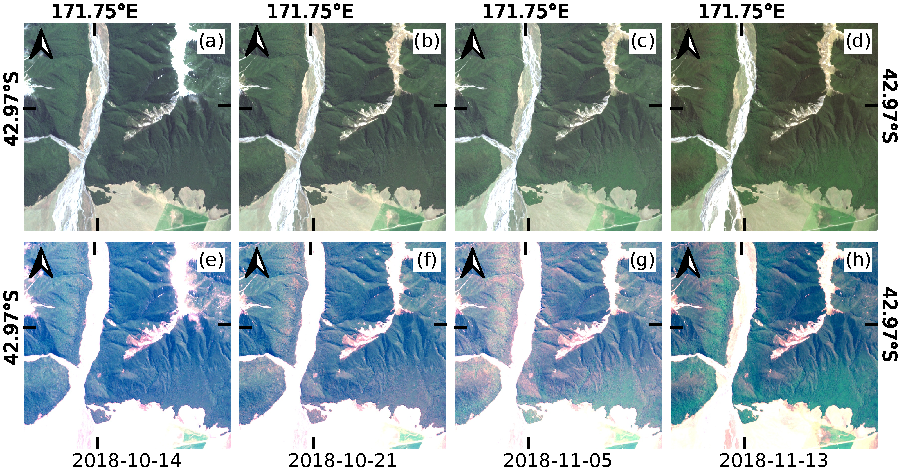
\includegraphics[width=\textwidth]{images/figure1_rgb.pdf}
    \caption{Sentinel-2 imagery from the Hawdon Valley, South Island, New Zealand showing a flowering event during Spring 2018. (a) - (d) are natural color, (e) - (h) are natural color with an exaggerated stretch to amplify the 'red' band (Band 4). Images are organized by column, e.g. (a) and (e) are natural color and stretched color, respectively, for date 2018-10-14.}
    \label{fig:rgb}
\end{figure}  

In order to detect the yellowing associated with southern beech flowering, we apply two approaches: the calculation of a normalized difference yellowing index (NDYI) to describe the red/green band relationship; and the modelling of this index over the time-series of the image archive to detect variations from the expected (non-flowering) state. The effect is subtle enough that the technique required is very sensitive to cloud and shadow contamination. Additional to the cloud masking performed above, 'invalid' pixels from the cloud mask (cloud/shadow/snow/water) were buffered by 30 pixels (300 m) and patches of 'valid' pixels smaller than 100 ha were re-classified 'invalid'. Extra spectral filtering was then used to mask remaining pixels too bright or dark to be forest (or useful): $\text{B}4_{red} < 650\text{, B}3_{green} < 900\text{, B}2_{blue} < 1000\text{, B}8_{NIR} > 1000\text{, B}4_{red} - \text{B}5_{red edge} < -1500$. The result was then further buffered by 3 pixels.

The NDYI is similar to the well-known normalized difference vegetation index (NDVI)\citep{Rouse1974}, using the 'red' (Band 4 ~665 +/- 15 nm) and 'green' (Band 3 ~560 +/- 18 nm) Sentinel-2 bands instead of 'near-infrared' and 'red'. It is also very similar to the green-red vegetation index (GRVI)\citep{Tucker1979,Motohka2010}, with the order of the bands merely reversed:

\begin{equation}
    NDYI = \frac{(\text{B4}_{red} - \text{B3}_{green})}{(\text{B4}_{red} + \text{B3}_{green})}
\end{equation}

The NDYI is calculated using the Level-1C TOA reflectance product re-projected to the New Zealand Transverse Mercator (NZTM) coordinate reference system (EPSG:2193) and with invalid pixels masked. As the NDYI represents the ratio of red-green, and both are affected similarly by transient atmospheric conditions, it will be negative over most areas of forest most of the time (i.e. when a pixel is 'green'), increasing to near or slightly above 0 during heavy flowering events. 

Substantial annual variation is present in TOA reflectance observations over forest due to climatic conditions, vegetation phenology (e.g. new leaves), and sun angle. The NDYI signal visually observed during flowering is subtle enough in the context of a year of data that setting simple thresholds is inadequate to produce a reliable result. Additionally, flowering can occur at different times during the spring season, depending on latitude and altitude \citep{Wardle1984,Allen2014}. The temporal sequence of NDYI for a pixel in the Hawdon Valley (South Island, New Zealand) is shown in Figure \ref{fig:sine} as an example. The orange line is a modelled NDYI time series unique to that pixel, using an approach similar to that used in the TMASK methodology developed for cloud detection in Landsat 8 imagery \citep{Zhu2014}. The model uses robust regression to calculate unique per-pixel ($i,j$) coefficients for sine and cosine terms for intra- ($a_{1,i,j}$, $a_{2,i,j}$) and inter-annual ($a_{3,i,j}$, $a_{4,i,j}$) variability as well as a constant term ($c{i,j}$), where $x$ is the number of days since the start of the temporal sequence, $T_{yr}$ is the number of days per year, and $T_{all}$ is the number of days in the sequence:

\begin{equation}
    \text{NDYI}_{mod}(i,j,x) = c_{i,j} + a_{1,i,j}sin(2\pi\frac{x}{T_{yr}}) + a_{2,i,j}cos(2\pi\frac{x}{T_{yr}}) + a_{3,i,j}sin(2\pi\frac{x}{T_{all}}) + a_{4,i,j}cos(2\pi\frac{x}{T_{all}})
\end{equation}

\begin{figure}[H]
    \centering
    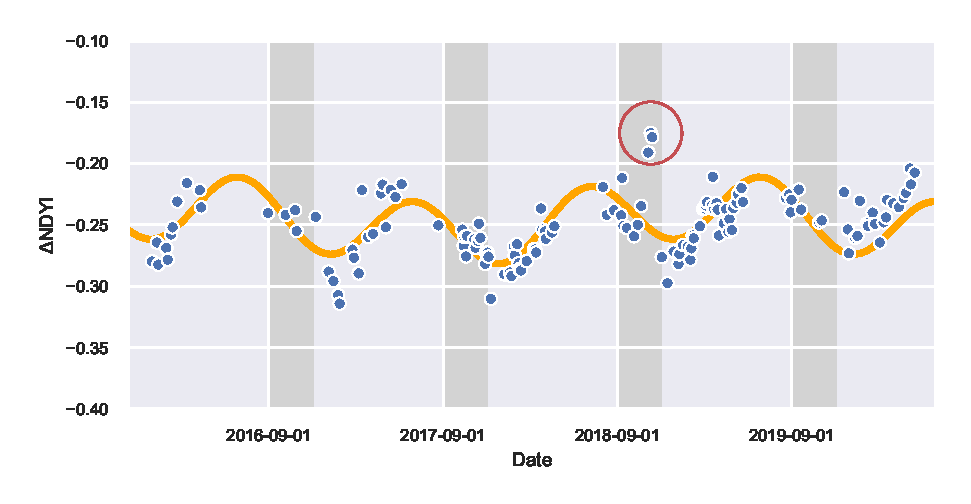
\includegraphics[width=\textwidth]{images/figure2_scatter_examplepixel_2018-2019.eps}%{images/figure1_ndyi_coeffs-windscreen_possibility_upscale.eps}
    \caption{Observed NDYI time series for an example pixel from Figure \ref{fig:rgb} in the Hawdon Valley (blue) with modelled values (orange) superimposed. Grey areas indicate austral spring seasons (September - November) where NDYI is expected to peak during a mast. Red circle shows higher-than-expected NDYI during spring 2018, the 'mega mast' season.}
    \label{fig:sine}
\end{figure}

Observed NDYI for each pixel/date were then subtracted from the modelled value for that pixel/date to produce \dndyi{} and the maximum value was found for each flowering season (September 1st to December 10th):

\begin{equation}
    \Delta\text{NDYI} = \text{NDYI} - \text{NDYI}_{mod}
\end{equation}

Finally, \dndyi{} values were converted to a map of 'heavy flowering detected' vs 'heavy flowering not detected' by following a method similar to \citet{Shepherd2007}. First, a high \dndyi{} threshold of 0.08 was chosen by assessing \dndyi{} against seed trap data \citep{Elliott2016} during the 2018 'mega mast'. This threshold was used to create 'seed' areas which were grown outwards by progressively lowering it to 0.04. The resulting 'flowering' pixels were then buffered by 2 pixels followed by a 5 x 5 majority filter then eroded by 2 pixels. 'Heavy flowering not detected' patches smaller than 1 ha (minimum mapping unit) were removed by re-coding as 'heavy flowering detected' or 'no data' (majority of surrounding pixels), then 'heavy flowering detected' patches smaller than 1 ha were re-coded 'heavy flowering not detected' to reduce small-scale noise. 

As no reliable spatial dataset of beech flowering exists beyond occasional field reports from DOC staff, the national-scale map for the 2018 mast year was accuracy-assessed by a human operator. At 1000 randomly selected sites, 500 in "heavy flowering detected" and 500 in "heavy flowering not detected", the operator determined whether heavy flowering was observed in a temporal sequence of 2018 cloud-free imagery in comparison with a median spring image (excluding 2018). Heavy flowering was easily observed in the temporal progression of spectral reflectance relative to the median image, especially when the spatial extent of flowering moved upward in elevation as the season progressed (using the exaggerated Red band stretch shown in Figure \ref{fig:rgb}). A confusion matrix of proportions was estimated using the method of \citet{Card1982}, from which precision and recall were calculated \citep{Maxwell2021}.

%%%%%%%%%%%%%%%%%%%%%%%%%%%%%%%%%%%%%%%%%%

\section{Results}

Austral spring (September/October/November) of 2017 was a light flowering season for southern beech in New Zealand. This was followed by a 'mega mast' in 2018 with heavy flowering observed from the ground during spring, and corresponding heavy seed fall the following autumn. Maps of maximum spring \dndyi{} were produced for each year of data, with results for the 2018 season shown in Figure \ref{fig:ndyinz}. Spatial patterns correspond with anecdotal reports from DOC staff based at field offices around New Zealand. There is heavy flowering throughout most of the north-western corner of the South Island, and sporadic heavy flowering in eastern Fiordland. The inset of Figure \ref{fig:ndyinz} highlights the level of detail available and shows heavy flowering on the lower slopes of the Hawdon and Poulter Valleys, dissipating as altitude increases up the valley walls (black areas are not beech forest - either alpine or riverbed in this location).

\begin{figure}
    \centering
    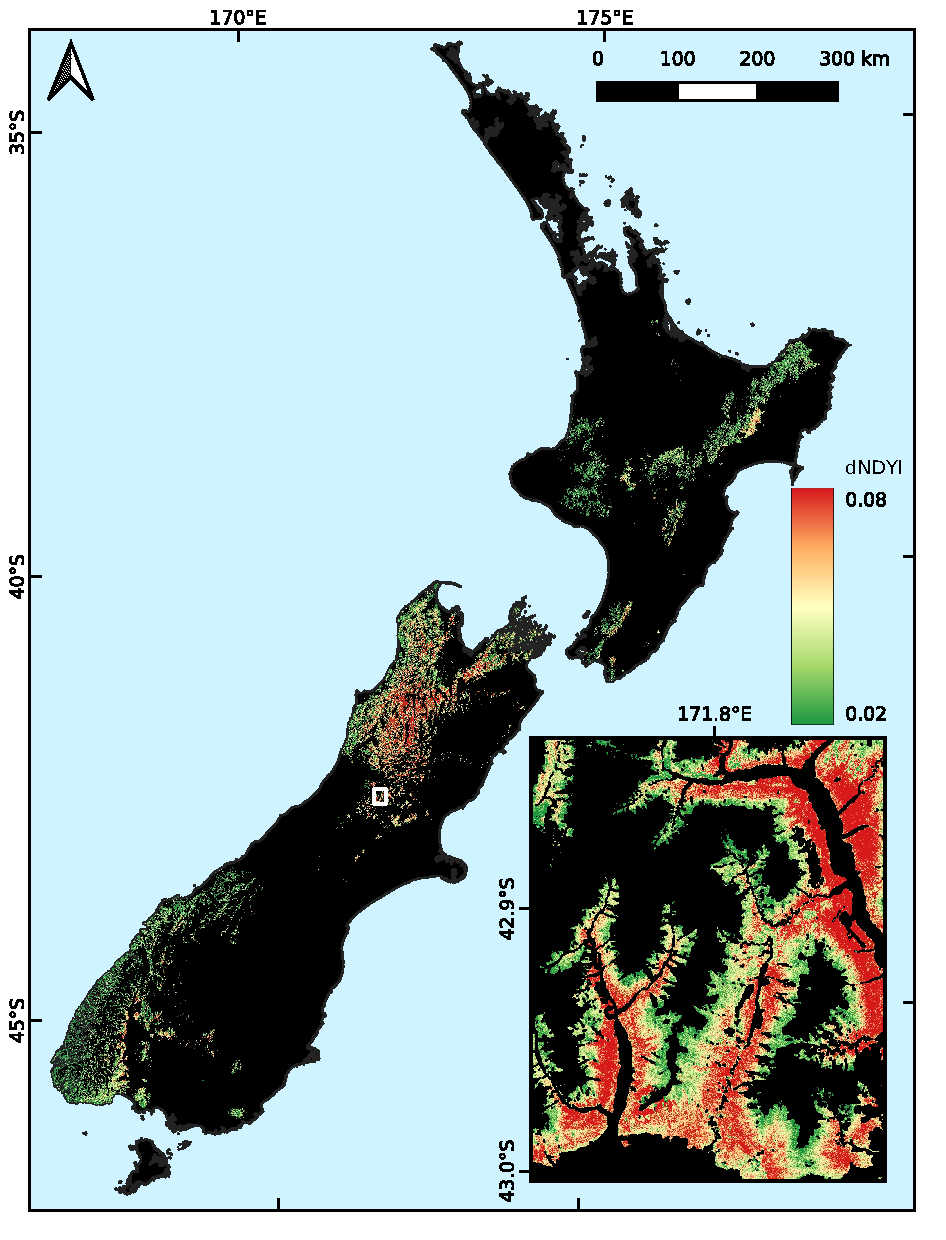
\includegraphics[width=\textwidth]{images/figure3_2018_dndyi.pdf}
    \caption{Maximum \dndyi{} (from modelled) for spring 2018 in areas of known southern beech forest in New Zealand. Green denotes areas of low (< 0.02) maximum \dndyi{}, while red is high (> 0.08) and indicates heavy beech flowering. Inset shows Hawdon and Poulter Valleys near Arthur's Pass (1:250,000 at 42.95\degree{}S, 171.82\degree{}E, see white box).}
    \label{fig:ndyinz}
\end{figure}  

Figure \ref{fig:mapts} shows the maps of heavy beech flowering as detected by the method for years 2017 through 2021. In spring 2018, much heavy beech flowering was detected in the north-west of the South Island, synonymous with a 'mega mast' event in that region. In the North Island and the south-west of the South Island, some pockets of heavy flowering were detected. The following year in spring 2019 the flowering was much reduced in the north-west of the South Island, but in the North Island much heavy flowering was detected, synonymous with another "mega mast". The south-west of the South Island had pockets of heavy flowering, much the same as in 2018. In years 2020 and 2021, minimal beech flowering was detected in most areas. 

\begin{figure}
    \centering
    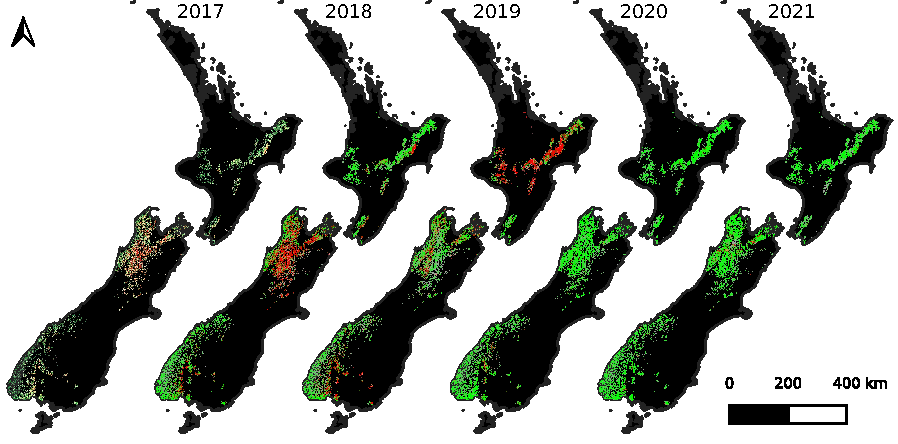
\includegraphics[width=\textwidth]{images/figure4_timeseries.pdf}
    \caption{Maps of heavy beech flowering during spring time for four years of Sentinel-2 imagery (2017 - 2021 inclusive). Classes are "heavy flowering detected" (red), "heavy flowering not detected" (green), and "no cloud-free imagery" (grey).}
    \label{fig:mapts}
\end{figure}  

In the 2018 map, heavy flowering was detected in 27.6\% (1144382 ha) of the 4.1 million ha of beech forest in New Zealand. Heavy flowering was not detected in 51.2\% (2122201 ha) of the beech forest. In the remaining 21.2\% of the beech forest (878406 ha) there was no cloud-free imagery in spring to make a decision. In each of the two classes, 'heavy flowering detected' and 'heavy flowering not detected', we generated 500 random locations at which we compared reference data with map data. Reference data were determined from visual interpretation of all the cloud-free spring imagery for the year. Table \ref{tab:confusion} shows the confusion matrix of proportions. Overall classification accuracy is 90.8\%. Precision (User's Accuracy) scores indicate that 90.4\% of the area mapped as 'heavy flowering detected' is actually heavy flowering. Recall (Producer's Accuracy) scores indicate that 84.4\% of actual 'heavy flowering detected' is successfully mapped as 'heavy flowering detected'. The overall F1 Score for 'heavy flowering detected' is 0.873, and 'heavy flowering not detected' is 0.928. Thus the \dndyi{} method is likely to under-estimate (slightly) rather than over-estimate areas of heavy flowering, however the scores reflect well on the method overall.

\begin{table}[H]
\centering
\caption{Confusion matrix showing detected/not detected heavy flowering (proportion of map) for the \dndyi{} method (Mapped) assessed against a human operator (Reference). Proportions are estimated from a random sample of 500 locations in 'heavy flowering detected' class (weighted by proportion of 'heavy flowering detected' in map = 0.35) and a random sample of 500 locations in 'heavy flowering not detected' class (weighted by 0.65). \label{tbl:confusion}}
%%% \tablesize{} %% You can specify the fontsize here, e.g., \tablesize{\footnotesize}. If commented out \small will be used.
\begin{tabular}{cc|cc|c}
\toprule
                                            &       & \multicolumn{2}{c}{\textbf{Reference flowering}}   & \\
	                                        &           & Detected  & Not Det.  & \textbf{Precision}\\
\midrule
\multirow{2}{*}{\textbf{Mapped flowering}}  & Detected	& 0.316		& 0.034     & 0.904 \\
                                            & Not Det.  & 0.059		& 0.592     & 0.910 \\
\midrule
    &                               \textbf{Recall}     & 0.844     & 0.946     &   \\
    &                               \textbf{F1 Score}   & 0.873     & 0.928     &   \\
%    &                               \textbf{Cohen's $\kappa$} & \multicolumn{2}{c}{0.797} & \\
\bottomrule
\end{tabular}
\label{tab:confusion}
\end{table}

%%%%%%%%%%%%%%%%%%%%%%%%%%%%%%%%%%%%%%%%%%

\section{Discussion}

We developed a method that produces a national map of heavy beech flowering from a temporal sequence of Copernicus Sentinel-2 imagery (Fig. \ref{fig:mapts}). The method detects elevated values of a yellow index, NDYI, above those normally expected in spring. A \dndyi{} value greater than 0.08 indicates especially heavy flowering, however these regions can be 'grown' into adjacent pixels where \dndyi{} is greater than 0.04 to better capture all heavy flowering. The elevated yellow index is caused by the production of red flowers obscuring green leaves. The national map of beech flowering may be produced at the end of spring, several months before the subsequent mast event actually occurs and seed drops to the ground. It is now provided to DOC, the national agency in charge of pest control, for planning additional pest control to be implemented several months later. In the 2018 spring, a nationwide beech mast event was detected and mapped by this method. A manual accuracy assessment determined the heavy flowering map to have an overall accuracy of  90\%. The spatial distribution of beech flowering as mapped by the method was also consistent with anecdotal observations from DOC field staff.

The national map of beech flowering can be used to provide extra detail to augment the existing $\Delta{T}$ model \citep{Kelly2013}, as it provides a higher spatial resolution of 10 m as opposed to 5 km. It is also a map of confirmed flowering, one less degree of separation from actual seed fall than the $\Delta{T}$ model, as physical factors such as carbon availability and soil moisture conditions also affect flowering and seed productivity \citep{Uscoe2005}. However, an issue with our method is the requirement for cloud-free satellite imagery at critical flowering times. This means that in some areas flowering may have been missed, which effectively makes the map a better indicator of ‘presence” rather than ‘absence’. 

\begin{figure}
    \centering
    % \includegraphics[width=\textwidth]{images/seeds_ndyi_201819.eps}
    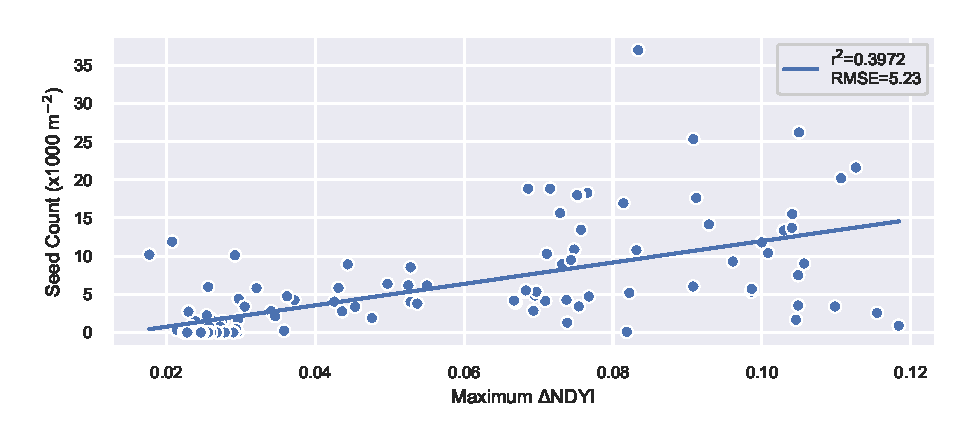
\includegraphics[width=\textwidth]{images/figure5_scatter_ndyi_seed_2018-2019.eps}
    \caption{Relationship between maximum \dndyi{} (spring 2018) and number of seeds collected from seed traps in the permanent trap network (autumn/winter 2019) for the 2018/19 masting season. Locations are filtered to exclude those with fewer than eight valid satellite observations.}
    \label{fig:trayscatter1819}
\end{figure}   

Not all heavy beech flowering in spring will result in heavy seed fall in the following autumn. Heavy frost or very wet weather can interfere with seed production \citep{Wardle1984}.  Figure \ref{fig:trayscatter1819} shows how well the maximum \dndyi{} compares with seed counts in trays located on the floor of beech forest (seed traps are spread throughout beech forests in New Zealand as part of a long-running monitoring programme conducted by DOC \citep{Elliott2016}). Data were restricted to locations with at least eight valid observations to obtain representation over the majority of the spring season. There is noise in the data, nevertheless high seed counts generally correspond with high maximum \dndyi{} ($r^2$ = 0.397). For reference, the $\Delta{T}$ model had $r^2$ values between 0.331 and 0.556 for the same species range \citep{Kelly2013} (that study used the older genus name \emph{Nothofagus}). Reasons for mismatches between \dndyi{} and seed count include: cloud coverage still obscuring the flowering event despite high revisits (low \dndyi{} vs high seed count); inaccurate trap location (variable impact on relationship); trap location relative to flowering trees combined with wind direction during seed fall (high \dndyi{} vs low seed count); different beech species (different relationship between \dndyi{} and seed count); climate, adverse weather events, and nutrient availability (lower seed count vs higher \dndyi{}); and inaccuracies in the method (addressed in accuracy assessment). We recommend the national map of flowering/not flowering be regarded as a map of potential high seed fall for initial planning purposes, to be confirmed later with additional information such as selected field observations. 

One way to address the paucity of valid observations is to add more data sources. As the technique developed in this study relies only on red, green, blue, and NIR (for quality control) wavelengths, it should be possible to include data from commercial satellite constellations with higher revisit rates but lower spectral range or resolution, such as the Planet\footnote{https://www.planet.com/} 'Dove' constellation. Adding freely available Landsat-8 data could also increase the probability of obtaining a valid observation at a critical time. Targeted aerial imaging campaigns could also provide valuable information in areas of known data paucity, particularly if they were informed by observations from field staff. This study has shown the resolution requirement is low by aerial imaging standards which would allow higher flight altitudes and larger image footprints, substantially reducing cost. Multiple studies have shown that fusion of these separate data sources is useful in remote sensing \citep{Bolton2020,Cheng2020,Thapa2021,Peng2021,Dixon2021,Moon2021Multiscale}, though the spatial complexity and rugged terrain of the beech forests in New Zealand is likely to reduce the utility of the coarse-resolution MODIS optical imagery.

This study successfully mapped the presence of heavy flowering in beech trees at large scale (greater than 4 million ha) using a visible change in canopy color. A similar study by \citet{Garcia2021} was less successful, but did show that moisture-based indices in the lead-up to a flowering or seed/cone event could provide additional information. \citet{Marcos2015} were also successful in predicting mast events using a combination of the enhanced vegetation index (EVI), and weather data during spring. A number of challenges exist in the context of detecting mast events, and the \dndyi{} approach attempts to minimize these. The NDYI index was chosen to specifically target red and green image bands, avoiding red-edge and near-infrared bands that also respond to vegetation condition and thus increase noise. The effectiveness of the multi-year sine and cosine model for modelling the typical behaviour of NDYI, the utilisation of extreme \dndyi{} values as 'seeds' for regions that grew into areas of lower \dndyi{} values, and the ability to tune spectral value constraints have all contributed to the effectiveness of our approach. To further improve the performance of the \dndyi{} method, it would be worth investigating the use of supporting indices like \citet{Garcia2021} and \citet{Marcos2015}, in addition to adding extra data sources. Further work distinguishing different beech species would add greater value to DOC as those with larger seeds (red and hard beech) have a disproportionately-larger impact on rodent irruptions.

Temporal analysis of Sentinel-2 satellite imagery has proved successful at detecting heavy flowering in New Zealand beech forests. To achieve this, cloud clearing had to be accurate (because the yellow index is sensitive to missed cloud) and automated (because many images are required). Automation of the cloud clearing \citep{Shepherd2020} and other processing means that beech flowering maps can be produced in a timely and cost-effective way. In future, we plan to produce a national map of heavy beech flowering at the end of each spring. This would give several months for analysis to plan the extra pest control required in autumn, improving the targeting of pest control in masting areas, and leading to better outcomes for native fauna.


%%%%%%%%%%%%%%%%%%%%%%%%%%%%%%%%%%%%%%%%%%
\section{Conclusions}
This study used Sentinel-2 top-of-atmosphere (TOA) imagery to detect and map atypical yellowing associated with heavy flowering of southern beech (\emph{Fuscospora} and \emph{Lophozonia}) in New Zealand over ~4.1 million ha at an unprecedented 10 m spatial resolution. This was achieved by modelling a normalized difference yellowing index (NDYI) over 5 years of observations and investigating deviations from expected values during spring months (September--November). A 'threshold' \dndyi{} value of 0.08 may be used to identify areas of heavy flowering, with connected areas of \dndyi{} > 0.04 also likely flowering. The method has been automated and can be run for all of New Zealand in less than a day on a cluster of approximately 1000 CPU cores. Using Sentinel-2 imagery, the method typically provides information on heavy flowering for 80\% of the beech forests in New Zealand with a high overall classification accuracy of 90.8\%, producing useful information for planning national-scale pest control efforts.


%%%%%%%%%%%%%%%%%%%%%%%%%%%%%%%%%%%%%%%%%%
\vspace{6pt} 

%%%%%%%%%%%%%%%%%%%%%%%%%%%%%%%%%%%%%%%%%%
%% optional \supplementary{The following are available online at \linksupplementary{s1}, Figure S1: title, Table S1:
%title, Video S1: title.}

% Only for the journal Methods and Protocols: If you wish to submit a video article, please do so with any other
% supplementary material. \supplementary{The following are available at \linksupplementary{s1}, Figure S1: title, Table
% S1: title, Video S1: title. A supporting video article is available at doi: link.}

%%%%%%%%%%%%%%%%%%%%%%%%%%%%%%%%%%%%%%%%%%
\authorcontributions{Conceptualization, Ben Jolly, John Dymond, Terry Greene, and Jan Schindler; Data curation, Ben Jolly, James Shepherd and Jan Schindler; Formal analysis, Ben Jolly; Funding acquisition, John Dymond; Investigation, Ben Jolly, John Dymond, and Terry Greene; Methodology, Ben Jolly, John Dymond, James Shepherd, and Terry Greene; Project administration, John Dymond; Resources, John Dymond; Software, Ben Jolly, James Shepherd and Jan Schindler; Supervision, John Dymond; Visualization, Ben Jolly; Writing – original draft, Ben Jolly; Writing – review \& editing, John Dymond, James Shepherd, and Terry Greene.}

%%%%%%%%%%%%%%%%%%%%%%%%%%%%%%%%%%%%%%%%%%
\funding{This research was funded by the New Zealand Ministry of Business, Innovation and Employment (MBIE) Endeavour Fund under the Advanced Remote Sensing of Aotearoa research programme (C09X1709).}

%%%%%%%%%%%%%%%%%%%%%%%%%%%%%%%%%%%%%%%%%%
\acknowledgments{The authors would like to thank the New Zealand Department of Conservation (DOC) for providing advice and validation data.}

%%%%%%%%%%%%%%%%%%%%%%%%%%%%%%%%%%%%%%%%%%
\conflictsofinterest{The authors declare no conflict of interest. The funders had no role in the design of the study; in the collection, analyses, or interpretation of data; in the writing of the manuscript, or in the decision to publish the results.} 

%%%%%%%%%%%%%%%%%%%%%%%%%%%%%%%%%%%%%%%%%%
%% optional
\abbreviations{The following abbreviations are used in this manuscript:\\

\noindent 
\begin{tabular}{@{}ll} 
DOC     & Department of Conservation \\
ESA     & European Space Agency \\
EVI     & Enhanced vegetation index \\
GRVI    & Green-red vegetation index \\
NDVI    & Normalized difference vegetation index \\
NDYI    & Normalized difference yellowing index \\
NZTM    & New Zealand Transverse Mercator \\
TOA     & Top of atmosphere\\



\end{tabular}
}

%%%%%%%%%%%%%%%%%%%%%%%%%%%%%%%%%%%%%%%%%%
% Citations and References in Supplementary files are permitted provided that they also appear in the reference list
% here. 

%=====================================
% References, variant A: internal bibliography
%=====================================
% \reftitle{References} \begin{thebibliography}{999} % Reference 1 \bibitem[Author1(year)]{ref-journal} Author1, T. The
% title of the cited article. {\em Journal Abbreviation} {\bf 2008}, {\em 10}, 142--149. % Reference 2
% \bibitem[Author2(year)]{ref-book} Author2, L. The title of the cited contribution. In {\em The Book Title}; Editor1,
% F., Editor2, A., Eds.; Publishing House: City, Country, 2007; pp. 32--58. \end{thebibliography}

% The following MDPI journals use author-date citation: Arts, Econometrics, Economies, Genealogy, Humanities, IJFS,
% JRFM, Laws, Religions, Risks, Social Sciences. For those journals, please follow the formatting guidelines on
% http://www.mdpi.com/authors/references To cite two works by the same author: \citeauthor{ref-journal-1a}
% (\citeyear{ref-journal-1a}, \citeyear{ref-journal-1b}). This produces: Whittaker (1967, 1975) To cite two works by the
% same author with specific pages: \citeauthor{ref-journal-3a} (\citeyear{ref-journal-3a}, p. 328;
% \citeyear{ref-journal-3b}, p.475). This produces: Wong (1999, p. 328; 2000, p. 475)

%=====================================
% References, variant B: external bibliography
%=====================================
\externalbibliography{yes}
\bibliography{library.bib}

\end{document}